\section{Results}\label{section:results}
\kant[5]

\subsection{Topic A}
\kant[10]

% =======================================================
\begin{equation}\label{eq:cannonical_partition_function}
Z=\sum _{i}e^{-\beta E_{i}}
\end{equation}
% =======================================================

\kant[11]

% =======================================================
\begin{figure}[h]\label{fig:test_single}
\begin{center}
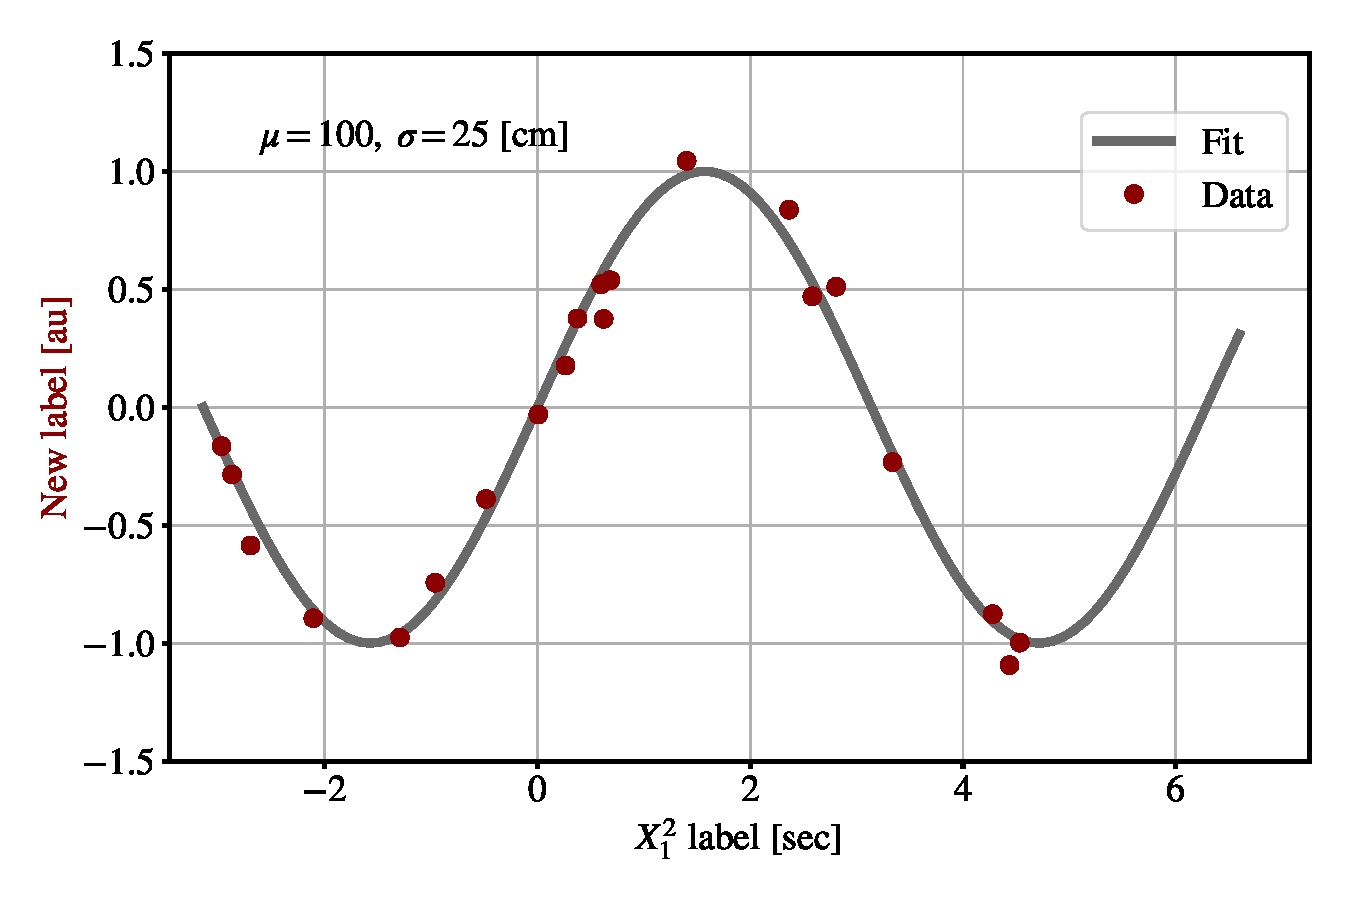
\includegraphics[scale=0.5]{figures/test_single.pdf}
\caption{This is a test figure.}
\end{center}
\end{figure}
% =======================================================

\kant[12-13] And there's more to be written about this topic.~\cite{einstein}

% =======================================================
\begin{table}[h]\label{tab:example_table}
\begin{center}\begin{tabular}{llr}
\toprule
\multicolumn{2}{c}{Item} \\
\cmidrule(r){1-2}
Number  & Description & Code \\
\midrule
1 & 6 & 87837 787 \\ 
 \hline
 2 & 7 & 78 5415 \\
 \hline
 3 & 545 & 778 7507 \\
 \hline
 4 & 545 & 18744 7560 \\
 \hline
 5 & 88 & 788 6344 \\ [1ex] 
\bottomrule
\end{tabular}\end{center}
\caption{Example table.}
\end{table}
% =======================================================

\kant[14]
